\documentclass{article}
\usepackage[T1]{fontenc}
\usepackage{lmodern}
\usepackage{graphicx}
\usepackage{amsmath,amssymb}
\usepackage[a4paper,margin=2cm]{geometry}
\usepackage[absolute,overlay]{textpos}
\setlength{\TPHorizModule}{1mm}
\setlength{\TPVertModule}{1mm}
\usepackage[indonesian]{babel}
\usepackage{hyperref}
\setlength{\emergencystretch}{2em}
% unit: Halaman 50

\begin{document}

% === Halaman 50 (llm) ===

\vspace{204.93mm}

Di bawah ini daftar 10.000 bilangan prima pertama (Sumber: http://primes.utm.edu):

\vspace{5mm}

% deskripsi: Daftar angka-angka bilangan prima yang disusun dalam format kolom
% bbox normalisasi: [0.0800, 0.1900, 0.8200, 0.8800]
\begin{textblock*}{155.40mm}(16.80mm,56.43mm)
\noindent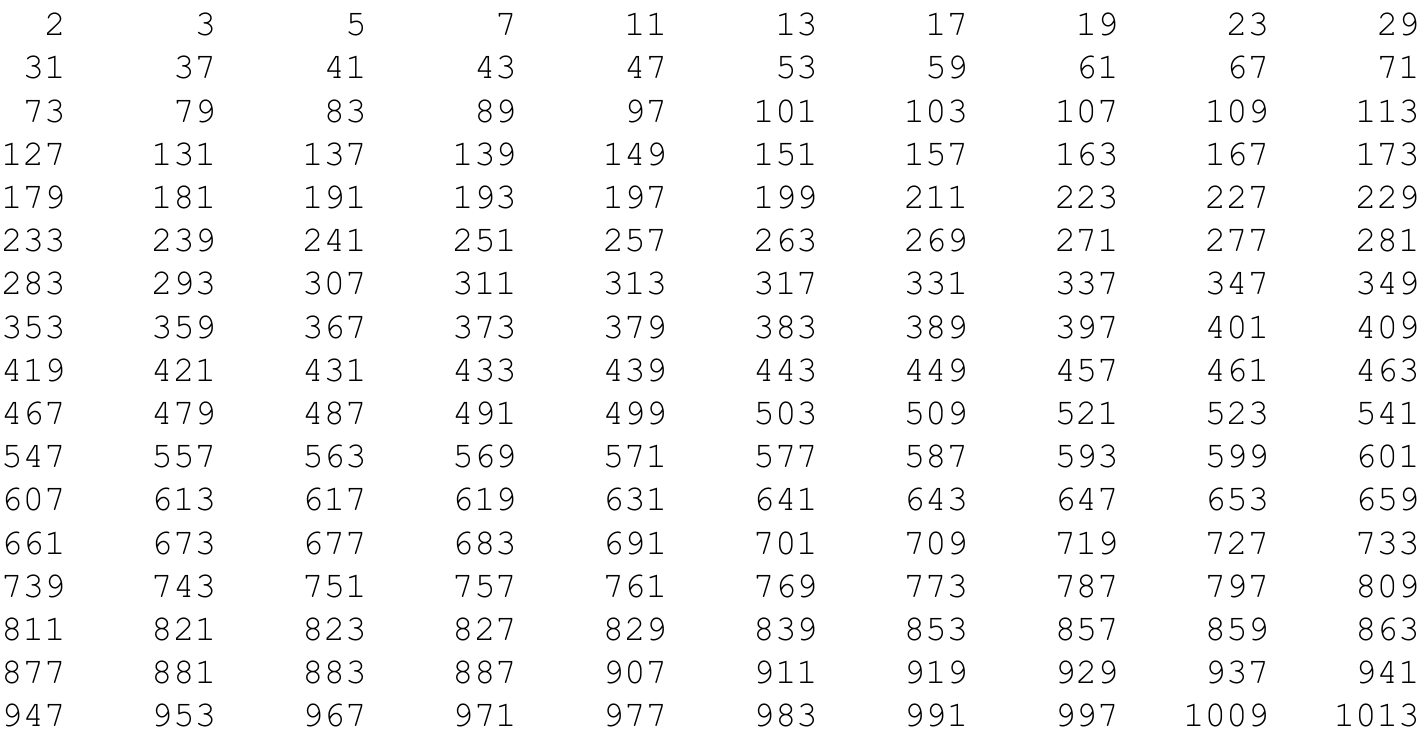
\includegraphics[width=155.40mm,height=204.93mm]{../../images/llm/page_050_img_01.png}%
\end{textblock*}

\end{document}
